\documentclass[10pt]{article}
\usepackage{mathpaper}

\begin{document}
\showsecret
\papertitle{2024年武汉市初中毕业生学业考试(模拟一)}
\mathtxt
\paperinformation
\centerline{\large \heiti 第Ⅰ卷 \quad 选择题(共30分)} \par \ \par

\begin{questions}{\selectingintroduction}
    \question 实数$14$的相反数是(~~~~~~~)
    \onp{$14$}{$-14$}{$\frac{1}{14}$}{$-\frac{1}{14}$}
    \question 图形美往往表现在对称当中,下列汉字中,是轴对称图形的是(~~~~~~~)
    \onp{\Huge \heiti 我}{\Huge \heiti 爱}{\Huge \heiti 中}{\Huge \heiti 国}
    \question 在一些比赛中,如果评委数多于两个人,往往会对评委们的打分进行``去掉一个最小值,再去掉一个最大值''的处理,这种处理方式一定不会改变原评分的(~~~~~~~)
    \onp{平均数}{中位数}{众数}{方差}
    \question 化简$(-4a^3)^3$的结果是(~~~~~~~)
    \onp{$-12a^{27}$}{$64a^{27}$}{$-12a^{9}$}{$-64a^{9}$}
    \question 由若干个同样大小的小正方体搭成的几何体的俯视图如图所示,其中小正方形中的数字表示在该位置小正方体的个数,则这个几何体左视图的面积是(~~~~~~~)
    \onp{$8$}{$9$}{$10$}{$11$}
    \question 已知在两个不透明的箱子甲和乙中分别装有几个除颜色外完全相同的小球,其中甲箱中有$2$个红球、$1$个黑球,乙箱中有$1$个红球、$1$个黑球.现通过掷硬币的方式随机抽取一个箱子,并在箱子中摸球,则下列说法中正确的是(~~~~~~~)
    \fop{若抽到了乙箱子,则随机摸一个球,摸出红球的概率更大}{若抽到了甲箱子,则随机摸两个球,一定能摸出黑球}{若在抽到的箱子中随机摸一个球,摸出的是黑球,则抽到乙箱子的概率更大}{若在抽到的箱子中随机摸两个球,则有可能摸出两个黑球}
    \question 已知两不等实数$a$、$b$满足$a^2-3a-1=0$、$b^2=3b+1$,则代数式$\frac{a^2+ab}{a-b} \div \frac{a^2b}{a^2-b^2}$的值是(~~~~~~~)
    \onp{$-9$}{$9$}{$-\frac{9}{4}$}{$\frac{9}{4}$}
    \question 已知在平面直角坐标系$xOy$中,一条平行于$x$轴的直线交$y$轴于正半轴,且分别交双曲线$y=-\frac{1}{x}$和$y=\frac{4}{x}$于点$A$、$B$,若$OA \bot OB$,则线段$AB$长(~~~~~~~)
    \onp{$\frac{5}{2}$}{$5$}{$\frac{5}{2}\sqrt{2}$}{$5\sqrt{2}$}
    \question 如图,$AB$是半圆$O$的直径,$C$是$\wideparen{AB}$的中点,$D$是$\wideparen{AC}$的中点,连$BD$、$BC$、$CA$、$CO$,设$DB$与$AC$的交点为$H$,与$OC$的交点为$G$,则有如下说法:\circnum{1}$CG=GH$;\circnum{2}$BC=2AD$;\circnum{3}$AB^2-DB^2=DH \cdot DB$;\circnum{4}$DH \cdot HB + \frac{1}{2}CH \cdot AC = CH \cdot AH.$其中正确的是(~~~~~~~)
    \onp{\circnum{1}\circnum{3}}{\circnum{2}\circnum{3}}{\circnum{1}\circnum{3}\circnum{4}}{\circnum{1}\circnum{2}\circnum{3}\circnum{4}}
    \begin{figure}[!htb]
        \centering
        \subfigure[(第5题)]{
        \begin{tikzpicture}[>=Stealth,scale=0.6]
            \tikzset{
                box/.style ={
                rectangle, %矩形节点
                minimum width =17pt, %最小宽度
                minimum height =17pt, %最小高度
                draw=black %边框颜色}
                }}
            \node[box] at (0,0) {$3$};
            \node[box] at (0,1) {$2$};
            \node[box] at (-1,0) {$4$};
            \node[box] at (1,0) {$1$};
            \node[box] at (-1,-1) {$2$};
            \node[box] at (1,-1) {$3$};
        \end{tikzpicture}}\qquad\qquad
        \subfigure[(第8题)]{
            \begin{tikzpicture}[>=Stealth,scale=0.6]
                \draw[->] (-2,0) -- (4,0) node[below] {$x$};
                \draw[->] (0,-1) -- (0,3) node[right] {$y$};
                \coordinate[label=below right:{$O$}] (O) at (0,0);
                \coordinate[label=above left:{$A$}] (A) at (-0.70711,1.41421);
                \coordinate[label=above right:{$B$}] (B) at (2.82843,1.41421);
                \draw[domain =-2:-1/3] plot (\x ,-1/\x);
                \draw[domain =4/3:4] plot (\x ,4/\x);
                \draw (O) -- (A) -- (B) -- cycle;
            \end{tikzpicture}
        }\qquad\qquad
        \subfigure[(第9题)]{
            \begin{tikzpicture}[>=Stealth,scale=0.5]
                \coordinate[label=below:{$O$}] (O) at (0,0);
                \coordinate[label=below:{$A$}] (A) at (-4,0);
                \coordinate[label=below:{$B$}] (B) at (4,0);
                \coordinate[label=above:{$C$}] (C) at (0,4);
                \coordinate[label=above left:{$D$}] (D) at (-2.82843,2.82843);
                \coordinate[label=below:{$H$}] (H) at (-1.65685,2.31345);
                \coordinate[label=above right:{$G$}] (G) at (0,1.65685);
                \draw (B) arc (0:180:4);
                \draw (A) -- (D) -- (B) -- (C) -- cycle;
                \draw (A) -- (B);
                \draw (O) -- (C);
            \end{tikzpicture}
        }
    \end{figure}
    \question 若整数$b$使得函数$t=x^2+bx+1$与函数$y=t^2+bt+1$没有相同的最小值,则这样的$b$有(~~~~~~~)个.
    \onp{$3$}{$4$}{$5$}{无数}
\end{questions}

\par \ \par \centerline{\large \heiti 第Ⅱ卷 \quad 非选择题(共90分)} \par \ \par

\begin{questions}{\complitingintroduction}
    \question 写一个比$3$大的无理数\complitingline
    \question {\kaishu ``2023年是共建`一带一路'倡议提出十周年。十年来,`一带一路'建设成就显著,中国企业在沿线国家建设的合作区已累计投资3979亿元人民币,为当地创造了42.1万个就业岗位。''}材料中数据``$42.1$万''可以用科学记数法表示为\complitingline (结果不带``万'')
    \question 一艘船在海上观测到一座灯塔位于东偏北$37^{\circ}$,在沿原方向继续行驶$1\text{n \ mile}$后,观测到这座灯塔位于东偏北$53^{\circ}$,则此时这艘船距离灯塔\complitingline n \ mile(结果四舍五入保留两位小数,参考数据:$\sin 37^{\circ} \approx 0.6$)
    \question 龟、兔进行$600$m赛跑,赛跑的路程$s$(m)与时间$t$(min)如图所示,若兔子睡觉前后速度保持不变,则当兔子到达终点时,乌龟已经到达了\complitingline min.
    \question 已知抛物线$y=ax^2+bx+c \ (a > 0)$经过$A(-1,1)$和$B(4,1)$两点,则有下列四个结论:
    \begin{subsubquestions}
        \subsubquestion $4a+c=1$;
        \subsubquestion 若点$C(\pi,y_0)$在抛物线上,则$y_0 < c$;
        \subsubquestion 若关于$x$的一元二次方程$ax^2+bx+c=0$有实数根$x_1$、$x_2 \ (x_1 \leq x_2)$,则$-1 < x_1 \leq x_2 < 4$;
        \subsubquestion 若关于$x$的一元二次方程$ax^2+bx+c=p$有实数根,则$4p \geq 4-25a$.
    \end{subsubquestions}
    其中正确的是\complitingline
    \question 如图,正方形$ABCD$中,$E$、$F$是$AD$上的两个动点(不与端点重合,$E$在$F$左侧也不与$F$重合),使得$AE=DF$,$CF$交$BD$于$G$,$BE$交$AG$于$H$,则$\frac{CH}{CE}$的取值范围是\complitingline

    \begin{figure}[!htb]
        \centering
        \subfigure[(第14题)]{
        \begin{tikzpicture}[>=Stealth,scale=0.45]
            \draw[->] (-1,0) -- (7,0) node[below right] {$t$/min};
            \draw[->] (0,-1) -- (0,7) node[above] {$s$/m};
            \node[below left] at (0,0) {$0$};
            \foreach \i in {1,2,...,6}
            {
                \draw (0,\i) -- (-0.1,\i) node[left] {$\i 00$};
            }
            \foreach \i in {1,2,...,6}
            {
                \draw (\i,0) -- (\i,-0.1) node[below] {$\i 0$};
            }
            \draw (0,0) -- (6,6) node[above left] {\kaishu 龟};
            \draw (0,0) -- (1,2) -- (5,2) -- (7,6) node[below right] {\kaishu 兔};
            \draw[densely dashed] (0,6) -- (7,6);
            \draw[densely dashed] (0,2) -- (1,2);
            \draw[densely dashed] (1,0) -- (1,2);
            \draw[densely dashed] (2,0) -- (2,2);
            \draw[densely dashed] (5,0) -- (5,2);
        \end{tikzpicture}}\qquad
        \subfigure[(第16题)]{
        \begin{tikzpicture}[>=Stealth,scale=0.5]
            \coordinate[label=above left:{$A$}] (A) at (0,6);
            \coordinate[label=below left:{$B$}] (B) at (0,0);
            \coordinate[label=below right:{$C$}] (C) at (6,0);
            \coordinate[label=above right:{$D$}] (D) at (6,6);
            \coordinate[label=above:{$E$}] (E) at (2.3,6);
            \coordinate[label=above:{$F$}] (F) at (3.7,6);
            \coordinate[label=below left:{$H$}] (H) at (2.00533,5.23129);
            \coordinate[label=right:{$G$}] (G) at (4.33735,4.33735);
            \draw (A) -- (B) -- (C) -- (D) -- cycle;
            \draw (B) -- (D);
            \draw (B) -- (E);
            \draw (A) -- (G);
            \draw (C) -- (H);
            \draw (C) -- (F);
            \draw (C) -- (E);
        \end{tikzpicture}}\qquad
        \subfigure[(第18题)]{
            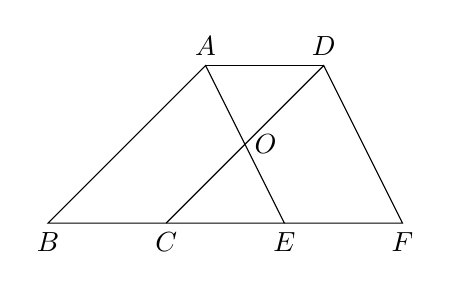
\begin{tikzpicture}[scale=0.5]
                \coordinate[label=below:{$B$}] (B) at (0,0);
                \coordinate[label=below:{$C$}] (C) at (3,0);
                \coordinate[label=below:{$E$}] (E) at (6,0);
                \coordinate[label=below:{$F$}] (F) at (9,0);
                \coordinate[label=above:{$A$}] (A) at (4,4);
                \coordinate[label=above:{$D$}] (D) at (7,4);
                \coordinate[label=right:{$O$}] (O) at (5,2);
                \draw (A) -- (B) -- (E) -- cycle;
                \draw (C) -- (D) -- (F) -- (E);
                \draw (A) -- (D);
            \end{tikzpicture}
        }
    \end{figure}
\end{questions}

\begin{questions}{\answeringintroduction}
    \question (本小题满分8分)\par
    解不等式组$\begin{cases}
        x+2 > -1 \ \text{\circnum{1}} \\
        3x-4 \leq x \ \text{\circnum{2}}
    \end{cases}$请按下列步骤完成解答:
    \begin{subquestions}
        \rmsubquestion 解不等式\circnum{1},得\complitingline
        \rmsubquestion 解不等式\circnum{2},得\complitingline
        \rmsubquestion 将不等式\circnum{1}和\circnum{2}的解集在数轴上表示出来:
        \addemptyline
        \begin{figure}[!htb]
            \centering
            \begin{tikzpicture}[>=Stealth,scale=1.2]
                \draw[->] (-4.3,0) -- (4.3,0);
                \foreach \i in {-4,-3,...,4}
                {
                    \draw (\i,0.1) -- (\i,0) node[below] {$\i$};
                }
            \end{tikzpicture}
        \end{figure}
        \rmsubquestion 原不等式组的解集为\complitingline
    \end{subquestions}
    \question (本小题满分8分)\par
    如图,四边形$ABCD$和四边形$ADEF$均是平行四边形,$AE$、$CD$交于点$O$,$AD=10$,$B$、$C$、$E$、$F$共线.
    \begin{subquestions}
        \subquestion 直接写出$\triangle ABE$可以怎样变换得到$\triangle DCF$.
        \subquestion 若$CE=10$,记$S_1$为$\triangle OCE$的面积,$S_2$为四边形$ABFD$的面积,求$\frac{S_1}{S_2}$.
    \end{subquestions}
    \question (本小题满分8分)\par
    主题班会课上,老师就同学之间如何相处,提出了四个观点:A.放下傲慢,彼此尊重;B.放下猜疑,彼此信任;C.相互支持,彼此成就;D.公平竞争,合作双赢. \par
    \qquad 老师要求每人选取一个观点写出自己的感悟,根据同学们的选择情况,学习委员绘制了下面两幅不完整的图表,请根据图表中提供的信息,回答下列问题:
    % \begin{figure}[!htb]
    %     \centering
    %     \subfigure{
    %         \begin{tabularx}{0.1635\textwidth}[!htb]{|c|c|c|} \hline
    %             观点 & 频数 & 频率 \\ \hline
    %             A & $a$ & $0.2$ \\ \hline
    %             B & $12$ & $0.24$ \\ \hline
    %             C & $8$ & $b$ \\ \hline
    %             D & $20$ & $0.4$ \\ \hline
    %         \end{tabularx}
    %     }\qquad
    %     \subfigure{
    %     \begin{tikzpicture}[>=Stealth,scale=0.1]
    %         \draw[->] (0,0) -- (45,0) node[below] {观点};
    %         \draw[->] (0,0) -- (0,30) node[right] {人数/人};
    %         \foreach \i in {5,10,...,25}
    %         {
    %             \draw[densely dashed] (40,\i) -- (0,\i) node[left] {$\i$};
    %         }
    %         \draw (5,0) -- (5,1);
    %         \draw (10,0) -- (10,1);
    %         \node[below] at (7.5,0) {A};
    %         \node[below] at (17.5,0) {B};
    %         \node[below] at (27.5,0) {C};
    %         \node[below] at (37.5,0) {D};
    %         \node[left] at (0,0) {$0$};
    %         \filldraw[color=white] (15,0) rectangle (20,12);
    %         \draw (15,0) rectangle (20,12);
    %         \filldraw[color=white] (25,0) rectangle (30,8);
    %         \draw (25,0) rectangle (30,8);
    %         \filldraw[color=white] (35,0) rectangle (40,20);
    %         \draw (35,0) rectangle (40,20);
    %         \node[above] at (17.5,12) {$12$};
    %         \node[above] at (27.5,8) {$8$};
    %         \node[above] at (37.5,20) {$20$};
    %     \end{tikzpicture}}
    % \end{figure}
    \begin{figure}[!htb]
        \centering
        \subfigure{
            \smallpicture{./images/table.png}{0.5}
        }\qquad \qquad
        \subfigure{
            \smallpicture{./images/barchart.png}{0.5}
        }
    \end{figure}
    \begin{subquestions}
        \subquestion 班里总共有\complitingline 人.
        \subquestion 表格中$a=$\complitingline,$b=$\complitingline
        \subquestion 将条形统计图补充完整.
        \subquestion 现准备从四个观点中任选两个作为演讲主题,请用列表或画树状图的方法求选中观点D(公平竞争,合作双赢)的概率.
    \end{subquestions}
    \question (本小题满分8分)\par
    如图,点$A$在直线$MN$的上方,过点$AB \bot MN$于$B$,$C$是射线$BN$上一点,使$BC < AB$,在$MN$的上方作$\angle ACD=\angle ACB$,以$CD$为直径的圆恰好经过点$A$且与$MN$交于点$E$.
    \begin{subquestions}
        \subquestion 求证:$AB$与这个圆相切.
        \subquestion 若$AB=2$、$CE=3$,试确定$\triangle ACD$的三边长.
    \end{subquestions}
    \begin{figure}[!htb]
        \raggedleft
        \subfigure[(第20题)]{
        \begin{tikzpicture}[>=Stealth,scale=0.5]
            \coordinate[label=below:{$B$}] (B) at (0,0);
            \coordinate[label=below:{$M$}] (M) at (-1.5,0);
            \coordinate[label=below:{$N$}] (N) at (6.5,0);
            \coordinate[label=below:{$C$}] (C) at (1,0);
            \coordinate[label=below:{$E$}] (E) at (4,0);
            \coordinate[label=left:{$A$}] (A) at (0,2);
            \coordinate[label=above right:{$D$}] (D) at (4,4);
            \draw (M) -- (N);
            \draw (B) -- (A) -- (C) -- (D) -- (E);
            \draw (A) -- (D);
            \draw (2.5,2) circle (2.5);
        \end{tikzpicture}}
    \end{figure}
    \question (本小题满分8分)\par
    如图是由小正方形组成的$9 \times 6$网格,每个小正方形的顶点被称为格点,在格点三角形$ABC$中,$P$是边$AB$上任意一点.仅用无刻度的直尺在给定网格中完成画图,画图过程用虚线表示.
    \begin{subquestions}
        \subquestion 在图1中,将线段$AB$沿$BC$方向平移,使点$B$与点$C$重合,画出平移后的线段$DC$,再在$DC$上画点$E$,使$CE=2AP$.
        \subquestion 在图2中,先在$AC$上画点$F$,使$\tan \angle ABF=\frac{3}{2}$,再在$AC$上画点$G$,使$\angle APG=45^{\circ}$.
    \end{subquestions}
    \begin{figure}[!htb]
        \centering
        \subfigure[(1)]{
        \begin{tikzpicture}[>=Stealth,scale=0.5]
            \draw[step=1,densely dashed] (0,0) grid (9,6);
            \coordinate[label=above:{$A$}] (A) at (6,6);
            \coordinate[label=right:{$B$}] (B) at (9,2);
            \coordinate[label=below:{$C$}] (C) at (6,0);
            \coordinate[label=right:{$P$}] (P) at (7.23,4.36);
            \draw (A) -- (B) -- (C) -- cycle;
            \filldraw (P) circle (0.05);
        \end{tikzpicture}} \qquad \qquad
        \subfigure[(2)]{
        \begin{tikzpicture}[>=Stealth,scale=0.5]
            \draw[step=1,densely dashed] (0,0) grid (9,6);
            \coordinate[label=above:{$A$}] (A) at (6,6);
            \coordinate[label=right:{$B$}] (B) at (9,2);
            \coordinate[label=below:{$C$}] (C) at (6,0);
            \coordinate[label=right:{$P$}] (P) at (7.23,4.36);
            \draw (A) -- (B) -- (C) -- cycle;
            \filldraw (P) circle (0.05);
        \end{tikzpicture}}
    \end{figure}
    \question (本小题满分10分)\par
    某课外科技活动小组研制了一种航模飞机,通过实验,收集了飞机相对于出发点的水平飞行距离$x$(单位:$m$)、飞行高度$y$(单位:$m$)随飞行时间$t$(单位:$s$)变化数据如下表:
    \begin{figure}[!htb]
        \centering
        \begin{tabularx}{0.5\textwidth}[!htb]{|m{3.8cm}<{\centering}|*{5}{>{\centering\arraybackslash}X|}} \hline
            飞行时间$t$(s)& $0$ & $2$ & $4$ & $8$ & $\dots$ \\ \hline
            水平飞行距离$x$(m)& $0$ & $20$ & $40$ & $80$ & $\dots$ \\ \hline
            飞行高度$y$(m) & $0$ & $31$ & $60$ & $112$ & $\dots$ \\ \hline
        \end{tabularx}
    \end{figure}
    \begin{enumerate}[topsep=0.5pt,parsep=0.5pt,itemsep=0.5pt,leftmargin=57.5pt,rightmargin=6pt]
        \item[\textbf{探究发现} \quad ] $x$与$t$、$y$与$t$之间的函数关系可以用我们已学过的函数来描述,直接写出$x$关于$t$的函数解析式和$y$关于$t$的函数解析式(不要求写出自变量的取值范围). \par
        \item[\textbf{问题解决} \quad ] 活动小组在水平安全线上$A$点处设置一个高度可以变化的发射平台试飞该航模飞机,现以$A$为原点、水平安全线为$x$轴、飞机飞行方向为正方向、$1$m为单位长度,建立平面直角坐标系.根据上面的 \ \textbf{探究发现} \ 解决下面的问题:
                                \begin{subquestions}
                                    \subquestion 若发射平台相对于安全线的高度为$0$m,在$A$点处持续发射激光,其轨迹可视为$y=\frac{8}{5}x$.若无人机在遇到激光$1$s后便发出信号,求航模发出信号时的坐标。
                                    \subquestion 在安全线上设置回收区域$MN$,使$AM=800$m,$AN=840$m.若飞机落到$MN$内(不包括端点),求发射平台相对于安全线的高度的变化范围。
                                \end{subquestions}
        \begin{figure}[!htb]
            \raggedleft
            \subfigure[(第22题)]{
                \begin{tikzpicture}[>=Stealth,scale=0.3]
                    \draw[->] (-0.5,0) -- (10,0) node[below] {$x$};
                    \draw[->] (0,-0.5) -- (0,5) node[right] {$y$};
                    \coordinate[label=below left:{$A$}] (A) at (0,0);
                    \draw (0,3) parabola bend (3,4) (8.5,0);
                    \draw[line width =1pt] (8,0) -- (9,0);
                    \coordinate[label=below:{$M$}] (M) at (8,0);
                    \coordinate[label=below:{$N$}] (N) at (9,0);
                \end{tikzpicture}}
        \end{figure}
    \end{enumerate}
    \question (本小题满分10分)\par
    \begin{enumerate}[topsep=0.5pt,parsep=0.5pt,itemsep=0.5pt,leftmargin=57.5pt,rightmargin=6pt]
        \item[\textbf{问题提出} \quad ] 如图1,在$\triangle ABC$中,$D$是线段$BC$中点,$F$是射线$AC$上一点,连$FD$并延长交$AB$于点$E$,探究$\frac{AB}{AE}$与$\frac{AC}{AF}$之间的关系.
        \item[\textbf{问题探究} \quad ]
                                \begin{subquestions}
                                    \subquestion 先将问题特殊化,如图2,当$\triangle ABC$为等边三角形,且$EF \bot AB$时,直接写出$\frac{AB}{AE}+\frac{AC}{AF}$的值.
                                    \subquestion 再研究一般情形,如图1,上述结论还成立吗?请给出证明.
                                \end{subquestions}
        \item[\textbf{问题拓展} \quad ] 在 \ \textbf{问题提出} \ 的基础上,将图1特殊化,如图3,$\angle ACB=90^{\circ}$,点$F$在线段$AC$上,连$AD$、$BF$交于点$G$,若$\angle CGD=90^{\circ}$、$\tan \angle FBC=\frac{\sqrt{6}}{7}$,求$\frac{AF}{FC}$所有可能的值.
    \end{enumerate}
    \begin{figure}[!htb]
        \centering
        \qquad\qquad
        \subfigure[(1)]{
        \begin{tikzpicture}[>=Stealth,scale=0.45]
            \coordinate[label=left:{$B$}] (B) at (0,0);
            \coordinate[label=above:{$A$}] (A) at (5,4);
            \coordinate[label=right:{$C$}] (C) at (6,0);
            \coordinate[label=below:{$D$}] (D) at (3,0);
            \coordinate[label=above left:{$E$}] (E) at (1.25188,1.00151);
            \coordinate[label=below right:{$F$}] (F) at (6.50151,-2.00603);
            \draw (A) -- (B) -- (C) -- cycle;
            \draw (A) -- (D);
            \draw (E) -- (F) -- (C);
        \end{tikzpicture}}\qquad\qquad
        \subfigure[(2)]{
        \begin{tikzpicture}[>=Stealth,scale=0.35]
            \coordinate[label=left:{$B$}] (B) at (0,0);
            \coordinate[label=above:{$A$}] (A) at (3,5.19615);
            \coordinate[label=right:{$C$}] (C) at (6,0);
            \coordinate[label=below:{$D$}] (D) at (3,0);
            \coordinate[label=above left:{$E$}] (E) at (0.75,1.29904);
            \coordinate[label=below right:{$F$}] (F) at (7.5,-2.59808);
            \draw (A) -- (B) -- (C) -- cycle;
            \draw (A) -- (D);
            \draw (E) -- (F) -- (C);
        \end{tikzpicture}}\qquad\qquad
        \subfigure[(3)]{
        \begin{tikzpicture}[>=Stealth,scale=0.6]
            \coordinate[label=left:{$B$}] (B) at (0,0);
            \coordinate[label=above:{$A$}] (A) at (6,4);
            \coordinate[label=right:{$C$}] (C) at (6,0);
            \coordinate[label=below:{$D$}] (D) at (3,0);
            \coordinate[label=right:{$F$}] (F) at (6,2.11675);
            \coordinate[label=above left:{$G$}] (G) at (4.08,1.44);
            \draw (A) -- (B) -- (C) -- cycle;
            \draw (A) -- (D);
            \draw (B) -- (F);
            \draw (C) -- (G);
        \end{tikzpicture}}\qquad\qquad
        \caption*{(第23题)}
    \end{figure}
    \question (本小题满分12分)\par
    在平面直角坐标系$xOy$中,抛物线$C_1$交$x$轴负半轴于$A$、正半轴于$B$,交$y$轴负半轴于$D$,使得$OB=OD=3OA=3$.
    \begin{subquestions}
        \subquestion 直接写出$C_1$的解析式.
        \subquestion 如图1,第一象限内$C_1$上有一点$F$,连$AF$、$BF$,若$\frac{1}{2}\angle AFB+\angle BAF=45^{\circ}$,求点$F$的坐标.
        \subquestion 如图2,将$C_1$平移得到$C_2$,使$C_2$的顶点为原点.$M$、$N$、$P$是抛物线上三点,其中$P$的横坐标为$1$,过$M$、$N$分别作不平行于$x$轴的直线交于点$E$,使直线$ME$、$NE$均与$C_2$有且仅有一个公共点.若$\triangle MPN$是以$P$为直角顶点的直角三角形,则点$E$是否在一条确定的直线上?若是,求这条直线的解析式;若不是,请说明理由.
    \end{subquestions}
    \begin{figure}[!htb]
        \centering
        \subfigure[(1)]{
        \begin{tikzpicture}[>=Stealth,scale=0.5]
            \draw[->] (-2,0) -- (5,0) node[below] {$x$};
            \draw[->] (0,-4.5) -- (0,2.5) node[right] {$y$};
            \coordinate[label=below right:{$O$}] (O) at (0,0);
            \coordinate[label=below left:{$A$}] (A) at (-1,0);
            \coordinate[label=below right:{$B$}] (B) at (3,0);
            \coordinate[label=left:{$D$}] (D) at (0,-3);
            \draw (-1.44949,2) parabola bend (1,-4) (3.44949,2);
            \coordinate[label=right:{$F$}] (F) at (3.23607,1);
            \draw (A) -- (F) -- (B);
        \end{tikzpicture}} \qquad \qquad
        \subfigure[(2)]{
        \begin{tikzpicture}[>=Stealth,scale=0.5]
            \draw[->] (-3,0) -- (4,0) node[below] {$x$};
            \draw[->] (0,-3) -- (0,4) node[right] {$y$};
            \coordinate[label=below right:{$O$}] (O) at (0,0);
            \coordinate[label=left:{$M$}] (M) at (-1.37239,1.88346);
            \coordinate[label=right:{$N$}] (N) at (1.68534,2.84038);
            \coordinate[label=above left:{$P$}] (P) at (1,1);
            \coordinate[label=below right:{$E$}] (E) at (0.15648,-2.31295);
            \draw (-2,4) parabola bend (0,0) (2,4);
            \draw (M) -- (N) -- (P) -- cycle;
            \draw (M) -- (E) -- (N);
        \end{tikzpicture}}
        \caption*{(第24题)}
    \end{figure}
\end{questions}
\end{document}